\documentclass[tikz,border=10pt]{standalone}
\usepackage{tikz}
\usepackage{pgfplots}
\usepackage{amsmath}
\usepackage{xcolor}
\usetikzlibrary{arrows.meta, positioning, decorations.pathreplacing}
\pgfplotsset{compat=1.18}

\tikzset{
    rdarrow/.style={red, thick, ->, >=Stealth},
    blarrow/.style={blue, thick, ->, >=Stealth},
    redtext/.style={font=\small, color=red, align=center},
    bluetext/.style={font=\small, color=blue, align=center, text width=8cm},
    distplot/.style={black, thick, domain=-2.5:2.5, samples=40}
}

\begin{document}
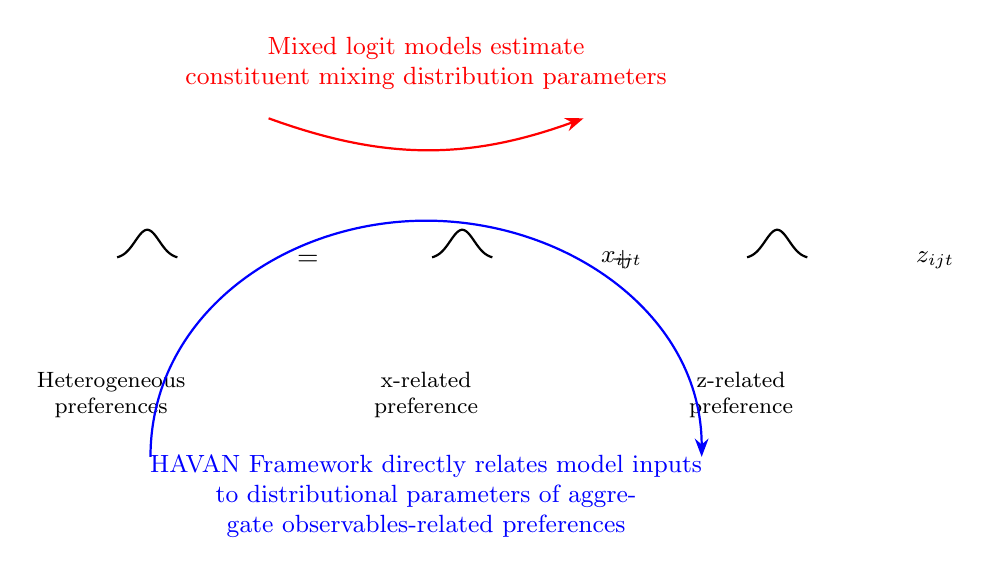
\begin{tikzpicture}[node distance=2.5cm and 3.5cm]

% 绘制三个正态分布
\foreach \x/\label/\var in {0/Heterogeneous\\preferences/, 4/x-related\\preference/$x_{ijt}$, 8/z-related\\preference/$z_{ijt}$} {
    \begin{scope}[shift={(\x,3)}]
        \begin{axis}[
            width=2.5cm, height=2cm,
            axis lines=none,
            domain=-2.5:2.5,
            samples=40
        ]
        \addplot[distplot] {exp(-x^2/2)/sqrt(2*pi)};
        \end{axis}
        \node[below=0.3cm, font=\footnotesize, align=center] at (0,-1) {\label};
        \ifx\var\empty\else
            \node[right=0.8cm, font=\small] at (1.3,0) {\var};
        \fi
    \end{scope}
}

% 上方红色标题和箭头
\node[redtext] at (4,5.5) {Mixed logit models estimate\\constituent mixing distribution parameters};
\draw[rdarrow] (2,4.8) to[bend right=20] (6,4.8);

% 添加加号和等于号
\node at (2.5,3) {$=$};
\node at (6.5,3) {$+$};

% 下方蓝色文字和箭头
\node[bluetext] at (4,0) {HAVAN Framework directly relates model inputs\\to distributional parameters of aggregate observables-related preferences};
\draw[blarrow] (0.5,0.5) to[out=90,in=180] (4,3.5) to[out=0,in=90] (7.5,0.5);

\end{tikzpicture}
\end{document}